\section{Auswertung}
\label{sec:Auswertung}

\subsection{Lange Spule}

\FloatBarrier

\begin{table}
\centering
\caption{Messwerte der langen Spule.}
\begin{tabular}{cc|cc}
  \toprule
  $x \:/\: \si{cm}$ & $B \:/\: \si{\milli\tesla}$ & $x \:/\: \si{cm}$ & $B \:/\: \si{\milli\tesla}$ \\
  \midrule
  -2.5 & 0.134 &  6 & 2.148  \\
  -2 & 0.162 & 12.5 & 2.203 \\
  -1.5 & 0.2 &  13 & 2.182 \\
  -1 & 0.254 & 13.5 & 2.160 \\
  -0.5 & 0.334 &  14 & 2.129 \\ 
  0 & 0.451  & 14.5 & 2.094 \\
  0.5 & 0.601 & 15 & 2.026 \\
  1 & 0.821  & 15.5 & 1.937 \\
  1.5 & 1.085  & 16 & 1.823 \\
  2 & 1.370  & 16.5 & 1.667 \\
  2.5 & 1.610  &  17 & 1.454 \\
  3 & 1.779  & 17.5 & 1.174 \\
  3.5 & 1.904  & 18 & 0.896 \\
  4 & 1.988 & 19 & 0.455 \\
  4.5 & 2.048  &  19.5 & 0.331 \\
  5 & 2.092  & 20 & 0.106 \\
  5.5 & 2.120 & & \\
  \bottomrule
\end{tabular}
\label{tab:long}
\end{table}

\begin{figure}
  \centering
  \caption{Das Magnetfeld der langen Spuele in Abhängikeit vom Ort in der Spule.}
  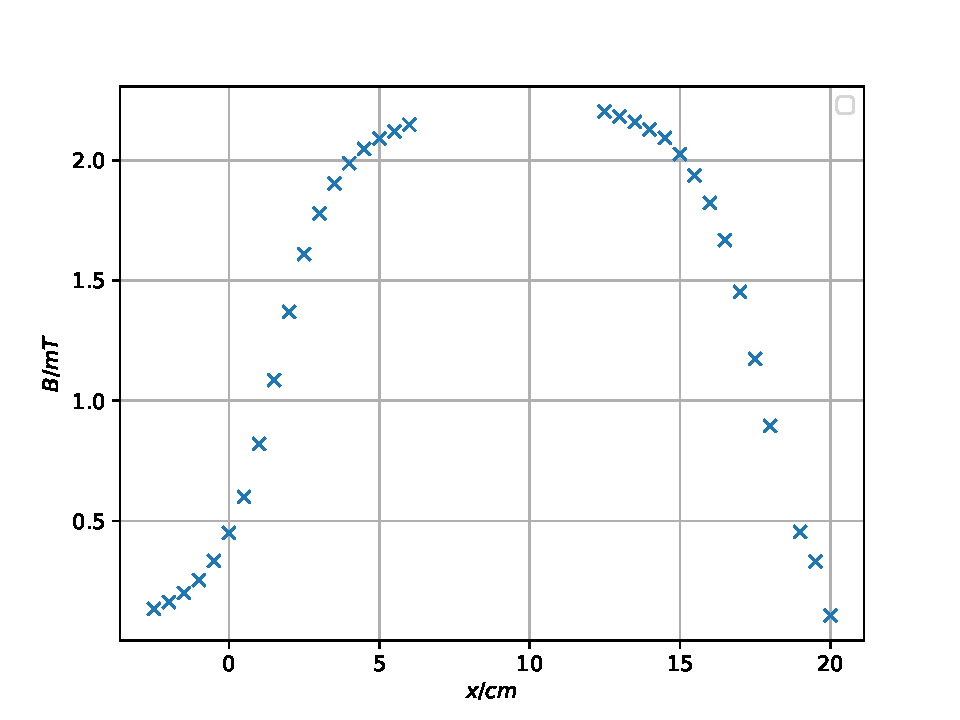
\includegraphics[width=\textwidth]{content/data/plot_long.pdf}
  \label{fig:long}
\end{figure}

In der Tabelle \ref{tab:long} sind die gemessen Werte aufgefasst.
Dabei steht $x=0$ für den Anfang der Spule.
In der Grafik \ref{fig:long} sind die Werte die in der Tabelle \ref{tab:long} aufgefasst sind, veranschaulicht dargestellt.

\FloatBarrier
\subsection{kurze Spule}

\begin{table}
\centering
\caption{Messwerte der kurzen Spule.}
\begin{tabular}{cc|cc}
\toprule
$x \:/\: \si{cm}$ & $B \:/\: \si{\milli\tesla}$ &$x \:/\: \si{cm}$ & $B \:/\: \si{\milli\tesla}$ \\
\midrule
-2.5 & 0.079 & 4.5 & 1.817  \\
-2 & 0.104 & 5 & 1.751  \\
-1.5 & 0.177 & 5.5 & 1.634  \\
-1 & 0.239 & 6 & 1.451  \\
-0.5 & 0.326 & 6.5 & 1.196  \\
0 & 0.465  & 7 & 0.937  \\
0.5 & 0.650  & 7.5 & 0.678  \\
1 & 0.905  & 8 & 0.488  \\
1.5 & 1.194  &  8.5 & 0.343  \\
2 & 1.430  & 9 & 0.237  \\
2.5 & 1.618  & 9.5 & 0.181  \\
3 & 1.750  & 10 & 0.137 \\
3.5 & 1.818  & 10.5 & 0.110 \\
4 & 1.837  & 11 & 0.087 \\
\bottomrule
\label{tab:short}
\end{tabular}
\end{table}

\begin{figure}
  \centering
  \caption{Die Messwerte aus der Tabelle \ref{tab:short} grafisch aufgefasst.}
  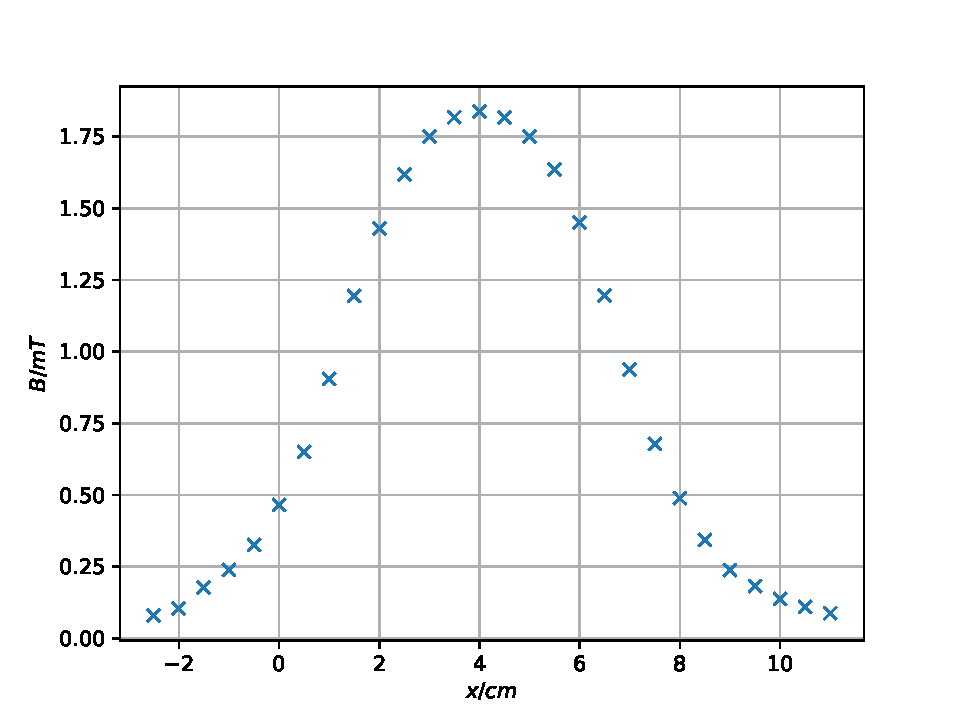
\includegraphics[width=\textwidth]{content/data/plot_short.pdf}
  \label{fig:short}
\end{figure}

Die Messwerte des Magnetfeldes der kurzen Spule sind in der Tabelle \ref{tab:short} zu sehen.
Die Werte sind anschließend in der Grafik \ref{fig:short} aufgetragen worden.
